\subsection{CLEMAP Client Dataset}

The client of CLEMAP operates within the Swiss printing and media industry where the equipment has been fitted with state of the art CLEMAP sensors on a range of their production equipment. The machines, location, and purpose are described in Table 1:

\begin{table}[htbp]
\scalebox{0.90}{
    \renewcommand{\arraystretch}{1.2}
    \centering
    \begin{tabular}{lcccccc}
    \hline
         Machine/Component & System & Amperes & Location & Floor & Purpose  \\
    \hline
    Gesamtmessung & & 1600 & Bau II & 0 & Main terminal \\
    Hauptluftung & HVAC & 250 & Bau II & -1 & Main ventilation \\
    Kältemaschiene & & 200 & Bau II & 1 & Refrigeration \\
    Drückmaschine & XL106 & 315 & Bau II & 2 & Printer \\
    UV Scan & XL106 & 160 & Bau II & 1 & undefined \\
    UV Sigmaline EG & & 315 & Bau II & 0 & undefined \\
    Stahl Folder & & 63 & Bau II & 0 & Steel folding \\
    Printer (Druckmaschine) & R707LV & 160 & Bau II & 2 & Printer \\
    Puderabsauger & R707LV & 25 & Bau II & 2 & Powder extraction \\
    Vari Air & R707LV & 100 & Bau II & 2 & undefined \\
    Trockner & R707LV & 160 & Bau II & 2 & Dryer \\
    UV Feinabgäng & & 125 & Bau II & 0 & UV fine particle extractor \\
    Papier Entsorgung & & 125 & Bau II & -1 & Paper disposal \\
    UV 1.0G & & 125 & Bau II & 1 & UV server room \\
    UV 2.0G & & 125 & Bau II & 2 & $2^{nd}$ floor \\
    UV 3.0G & & 125 & Bau II & 3 & $3^{rd}$ floor \\
    UV 4.0G & & 160 & Bau II & 4 & $4^{th}$ floor \\
    UV EG & & 125 & Bau II & 0 & UV ground floor \\
    \hline
    \end{tabular}}
    \caption{List of items being metered by CLEMAP. A system may be composed of several machines, all of which are being metered.}
    \label{tab:tab1}
\end{table}

All machines and the main terminals are connected to an \ac{a.c} grid with three phases. Subsequently, the data collected is the \ac{L}, V, I, W, \ac{p.f.}. The measurements were originally collected at a frequency of $12$Hz from October $7^{th}$ until October $18^{th}$ for a total length of $10$ days. A three phase current at $12$Hz indicates that every second, there should be $12$ cycles being measured for each phase $1, 2$ and $3$. 

As outlined in \hyperlink{subsection.3.3}{Section 3.3}, and due to the GPyTorch Gaussian Process time complexity of $\mathcal{O}(n^2)$, the time series is discretized by aggregating the data into $10$ and $30$ minute intervals and taking the average value. This aggregation significantly reduces the length of the original $12$Hz time series while still allowing for a more granular level of analysis compared to the current literature in \hyperlink{section.2}{Section 2}.

\subsubsection{CLEMAP Exploratory Data Analysis}

Here, an introductory EDA is performed on some of the machines and components that will be modeled in \hyperlink{section.5}{Section 5}. First, a bar plot broken down by machine energy consumption and hour of the day for the $10$ days is visualized for a general overview of the measurement setup.

\begin{figure}[htp]
\centering
\graphicspath{ {./images/} }
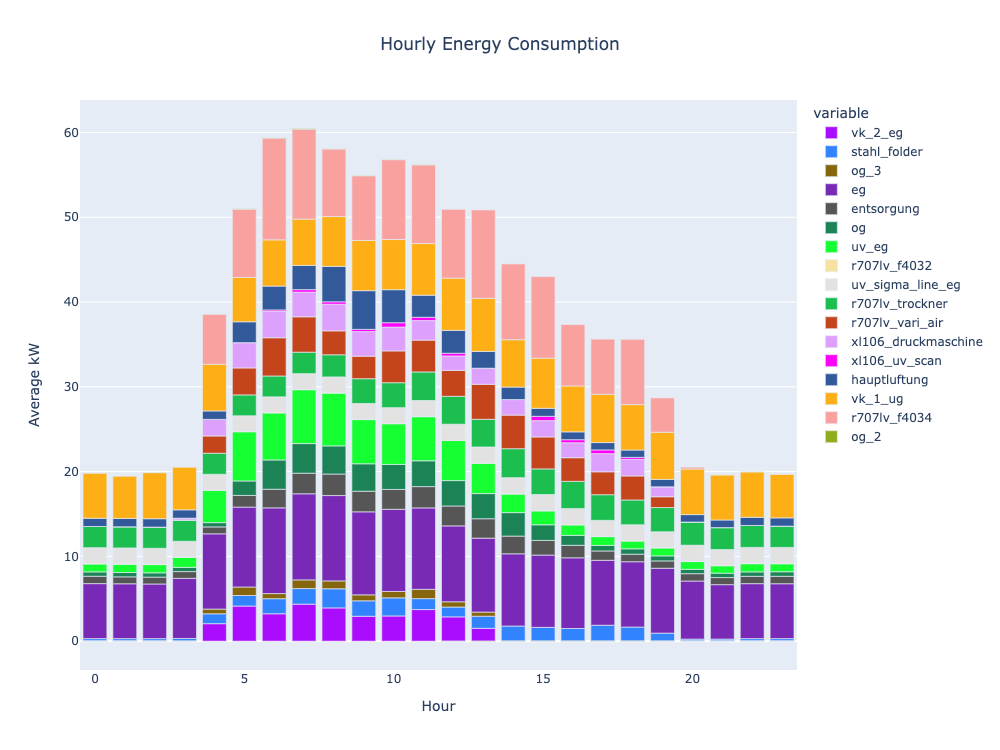
\includegraphics[scale=0.47]{images/hourly_load_barplot.png}
\caption{CLEMAP sensor measurement setup. Hourly load energy consumption (kWh) for each machine over the course of $10$ days.}
\label{fig:fig6}
\end{figure}

Using the meta data from Table \ref{tab:tab1} and the bar chart above, it is evident that machines on the ground, first, and second floor affect the energy being metered on their respective floors (UV 1.0G, etc.). Likewise, the meter on the main terminal is measuring all of the energy. The majority of the components being metered, with the exception of the Trockner, UV Sigmaline EG and VK 1.UG, are effected by the hour of the day. In the system R707LV, the printer demanded little to no energy, while the remaining three components represent a large share of total energy demanded with the powder extraction machine consuming the most. Subsequently, in the XL106 system, the printer represents the majority of energy demanded by the system. 

For the sake of brevity, only the EDA for the paper disposal machine (Figure \ref{fig:fig7}) will be shown below. For a full machine analysis, please refer to the \path{eda} directory on the \path{experiments} branch of the GitHub repository \cite{Stechschulte_Gaussian_Processes_for_2022}. 

\begin{figure}[h]
  \centering
  \graphicspath{ {./images/} }
  \subfloat[Outside of machine.]{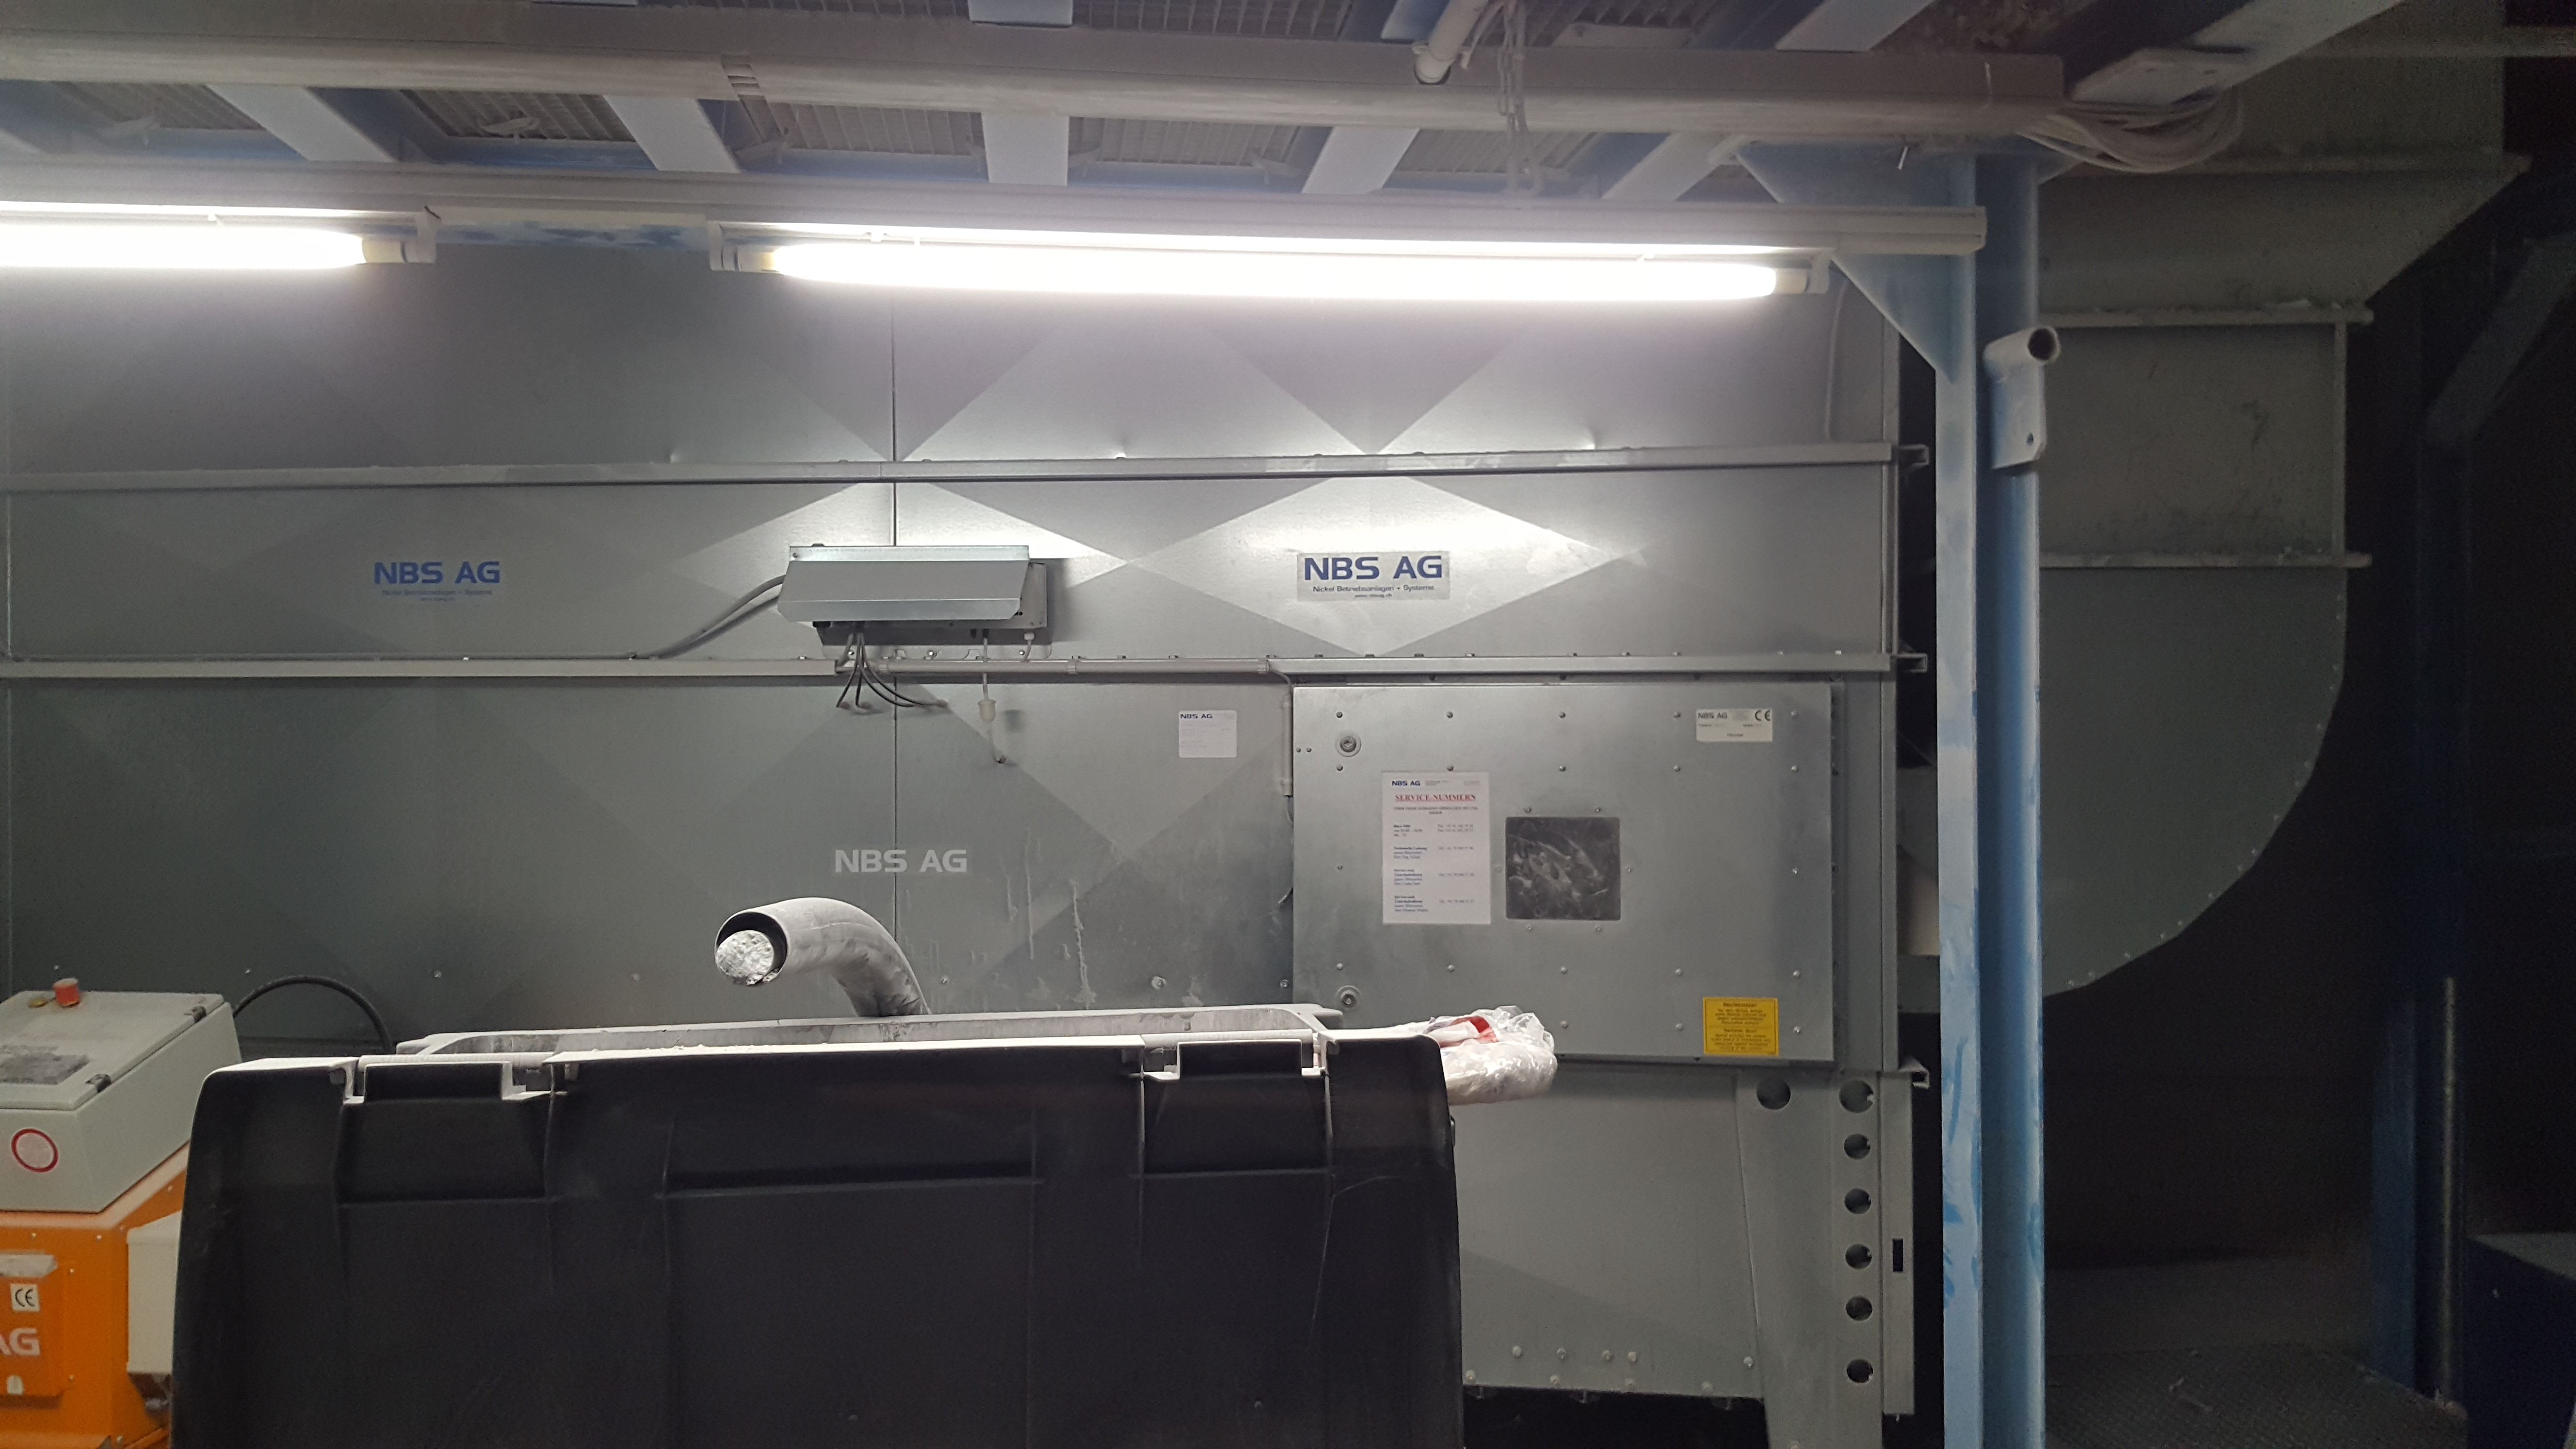
\includegraphics[width=0.4\textwidth]{images/papier_entsorgung_1.jpg}\label{fig:a7}}
  \hfill
  \subfloat[Output of machine.]{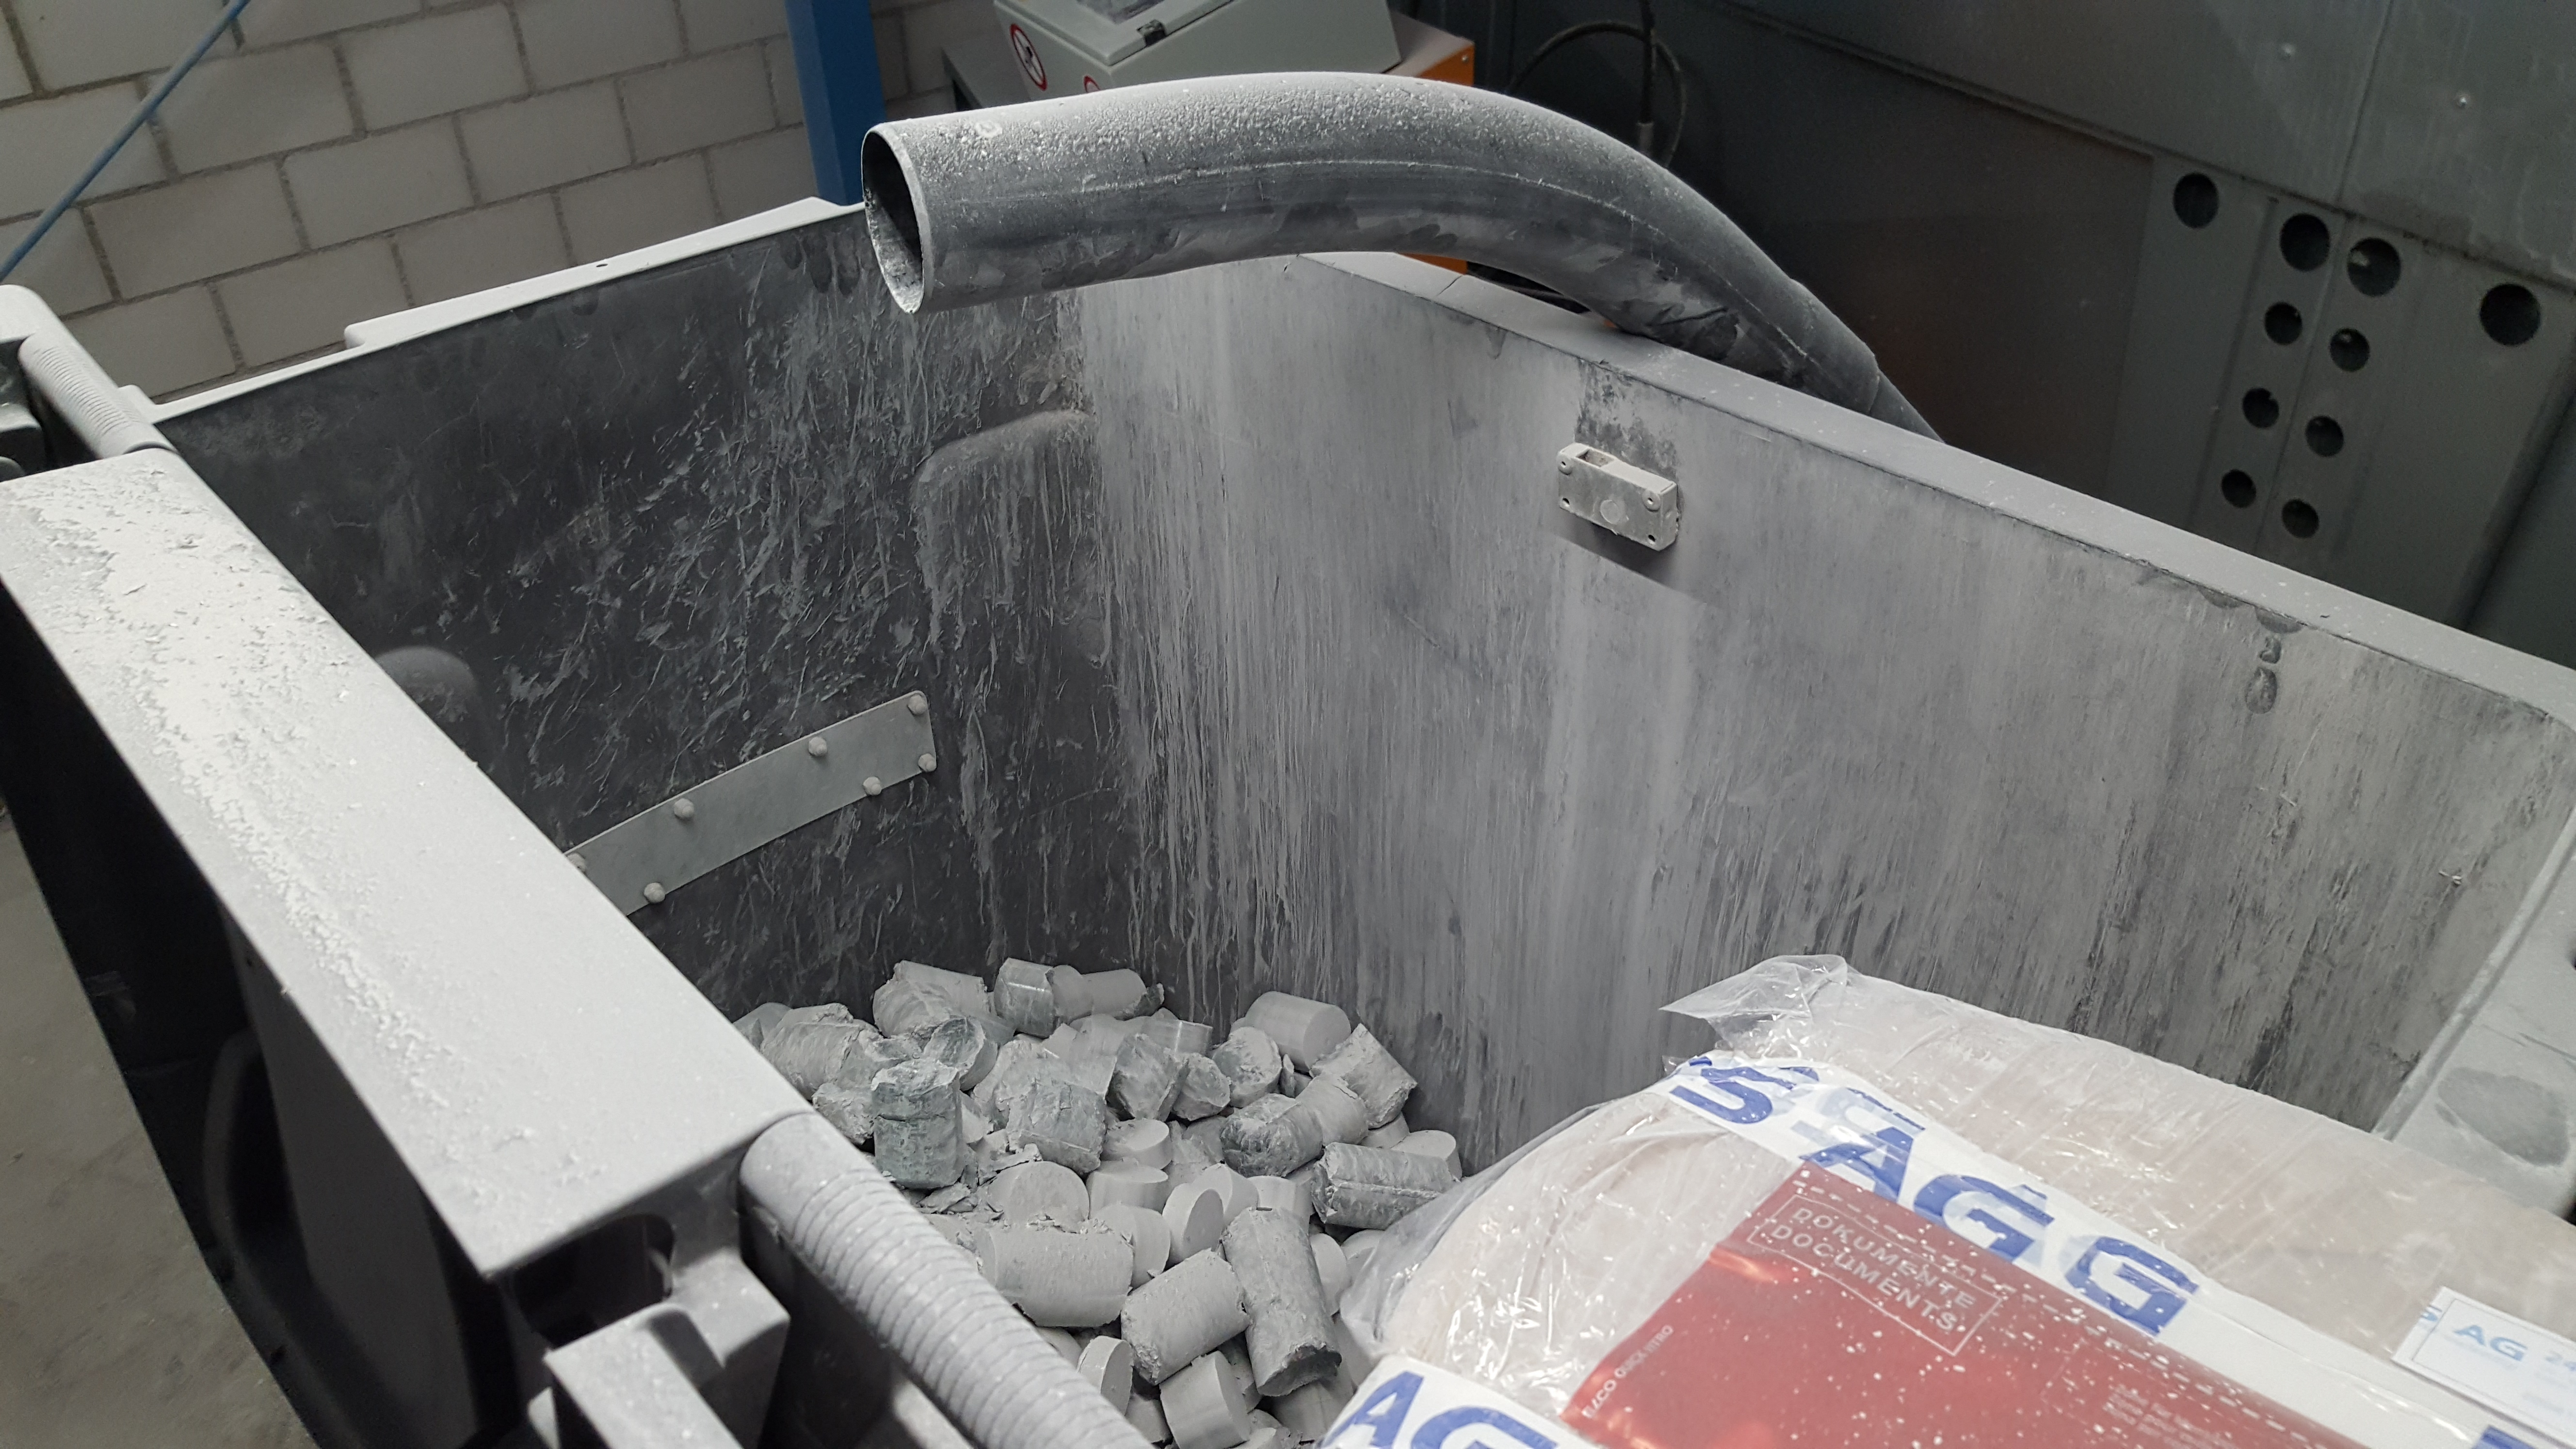
\includegraphics[width=0.4\textwidth]{images/papier_entsorgung_2.jpg}\label{fig:b7}}
  \caption{Paper disposal machine}
  \label{fig:fig7}
\end{figure}

Building off of the bar plot visualizations above and the characteristics of time series in \hyperlink{subsection3.3}{Section 3.3}, it is likely that the paper disposal machine has a cyclical pattern. Figure \ref{fig:fig8} is an hourly load profile heat map of the paper disposal machine. It is evident there is a daily periodicity from Monday to Friday with little to no demand on the weekend. The heat map indicates a daily and potential weekly pattern; though more data is needed to confirm the weekly periodicity hypothesis. 

\begin{figure}[h]
\centering
\graphicspath{ {./images/} }
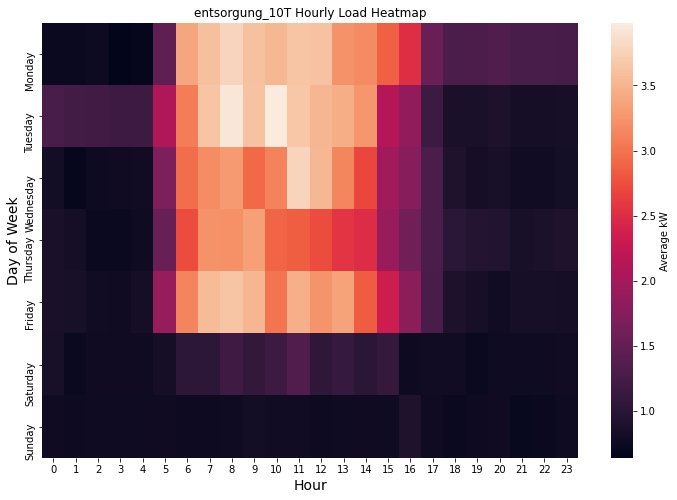
\includegraphics[scale=0.55]{images/entsorgung_hourly_heatmap.png}
\caption{Paper disposal hourly load profile. The color bar on the right indicates the average kW consumed for that hour over the $10$ day period.}
\label{fig:fig8}
\end{figure}

Next, in Figure \ref{fig:fig9}, a plot of the time series at a $10$ minute interval is visualized where 2021-10-08 is a Friday and 2021-10-18 is a Monday. The load profile shows a daily, and potentially sub-daily periodic pattern. Also, the $10$ days of data does not split into an even two weeks of data. Rather, there is only observations for one full production week. This inconsistency does not allow for an analysis or modeling of the weekly periodicity. 

\begin{figure}[H]
\centering
\graphicspath{ {./images/} }
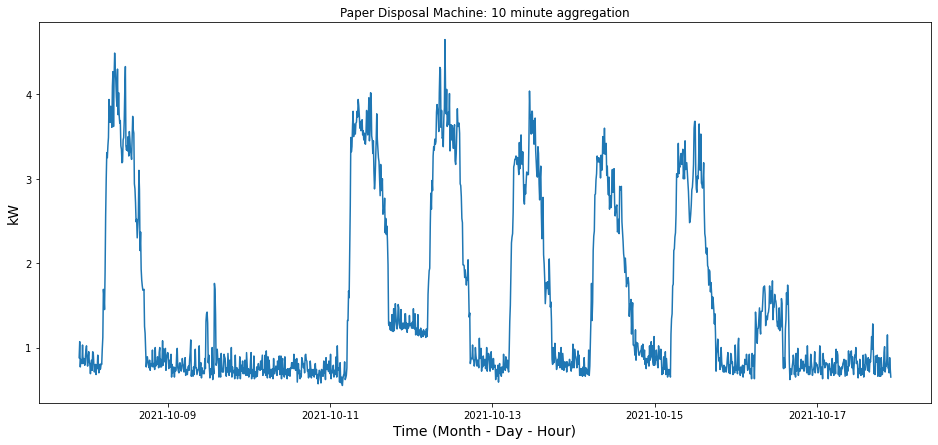
\includegraphics[scale=0.49]{images/entsorgung_10T_series.png}
\caption{Entire time series for the paper disposal machine.}
\label{fig:fig9}
\end{figure}

Therefore, during the modeling phase, only the production week (2021-10-11 through 2021-10-15) is used. Using this time series, the periodicity is verified empirically using the ACF; as explained in \hyperlink{subsubsection.3.5.3}{Section 3.5.3}. Below, in Figure \ref{fig:fig10}, the production week time series is visualized along with the respective ACF correlogram. Looking at the ACF and time series plot, the sub-daily and daily periodicity is verified at about $12$ and $24$ hours, respectively. Also, on some days, such as the $11^{th}$, $13^{th}$ and $14^{th}$, the load profile slowly tapers off compared to the other days. Furthermore, during non-operational hours, the machine seems to be ``on" and in a ``stand-by" mode.  

\begin{figure}[H]
    \centering
    \graphicspath{ {./images/} }
    \subfloat[a][a]{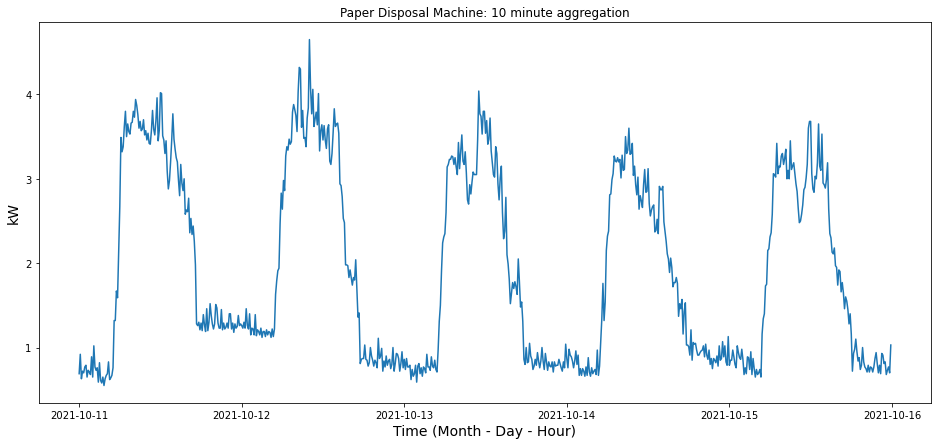
\includegraphics[width=1\textwidth]{images/entsorgung_10T_production_week.png}\label{fig:a10}} \\
    \subfloat[b][b]{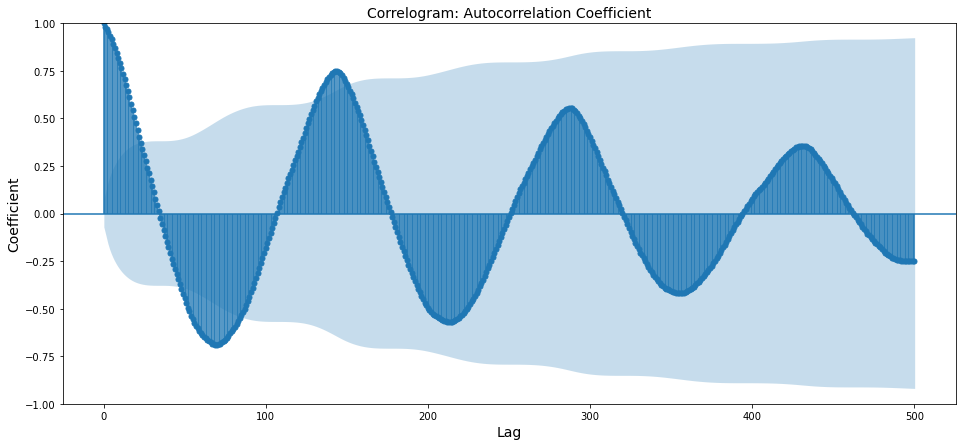
\includegraphics[width=1\textwidth]{images/entsorgung_10T_acf.png}\label{fig:b10}}
    \caption{(a) Production week time series at $10$ minute aggregations. (b) ACF correlogram indicates significant periodic cycles at about $12$ and $24$ hours, respectively. For example, $(75*10) / 60 = 12.5$} 
    \label{fig:fig10}
\end{figure}

Finally, the original time series is split into random, shorter time samples to gain a better visual understanding of the original $12$Hz frequency and cycle patterns. Indeed, in Figure \ref{fig:fig11}, a repeating cyclical pattern is identified during for, what could be called a ``stand-by" state, the non-operational time of the machine from 17:30 on October $11^{th}$ until 05:00 on October $12^{th}$. Subsequently, (b) the duration of the peak load, shows a less identifiable cycle. 

\begin{figure}[H]
    \centering
    \graphicspath{ {./images/} }
    \subfloat[a][a]{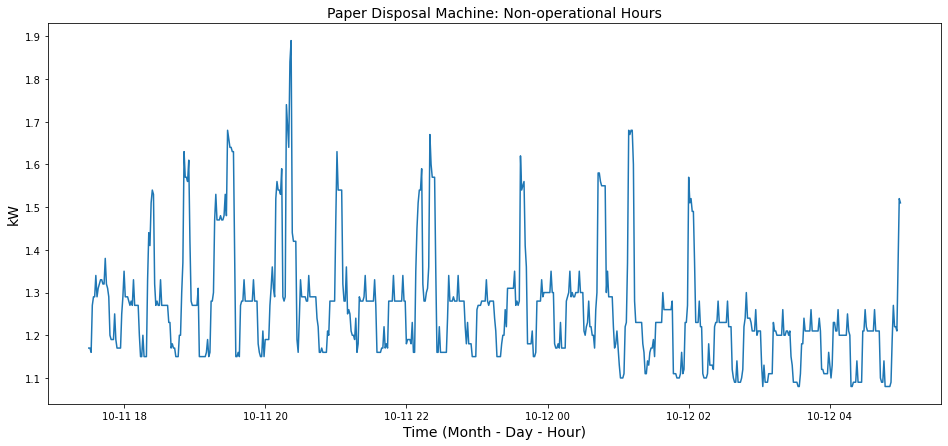
\includegraphics[width=1\textwidth]{images/non_operational_hours.png}\label{fig:a11}} \\
    \subfloat[b][b]{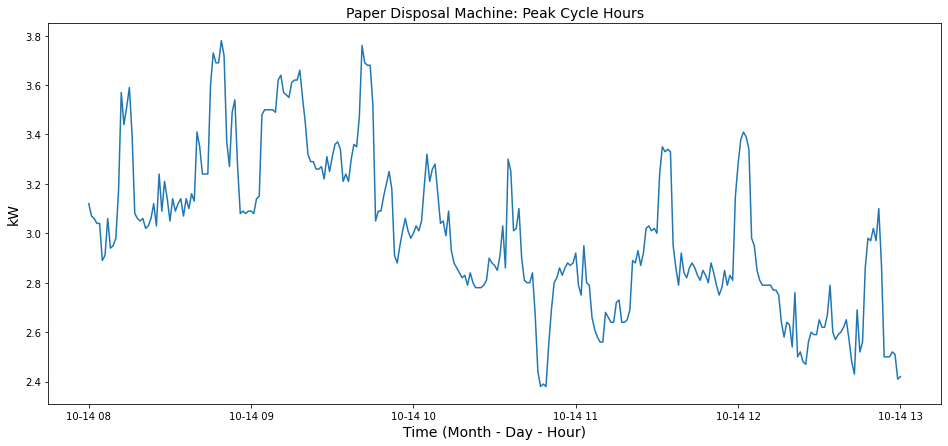
\includegraphics[width=1\textwidth]{images/peak_cycle_hours.png}\label{fig:b11}}
    \caption{(a) Random profile of non-operational hours from 17:30 - 05:00 (b) Random peak load profile from 08:00 - 13:00}
    \label{fig:fig11}
\end{figure}


\subsection{HIPE Industrial Energy}
Complementing CLEMAP's client machine-level data, a second source of data, the \ac{HIPE} energy status data set \cite{HIPE}, will also be analyzed to ensure the scalability of the proposed methodologies in section 4. By developing the algorithms on a range of industrial equipment, the methods developed in this thesis can give vital feedback on the difficulties and opportunities of the scalability and feasibility of models built on specific data sets to new data of similar applications. 

The HIPE data set comes from the \ac{IPE} of \ac{KIT} in Germany which operates an electronics production site. It produces electronic systems for particle physics, battery systems, and medical applications in small batches, i.e., less than 1,000 pieces. Several machines have been instrumented with smart meters in which the machines are either connected to one phase or three phase power. The machines and their purpose are outlined in Table \ref{tab:tab2} below.

\begin{table}[htp]
\scalebox{0.95}{
    \renewcommand{\arraystretch}{1.2}
    \centering
    \begin{tabular}{p{5cm}p{11cm}}
    \hline
         Machine/Component & Purpose  \\
    \hline
    Pick and place unit & Placement of electronic components, such as resistors and microcontrollers, on a printed circuit board (PCB). Energy consumption depends on the quantity of components per PCB and on the number of boards \\
    Soldering oven & Components soldering to PCB. Energy consumption depends on throughput speed and temperature \\
    Washing machine & Cleaning of PCB. Energy consumption depends on temperature and process duration \\
    Screen printer & Printing of material layers to interconnect electronic components via thick-film technology \\
    Vacuum Pump 1 & Auxiliary machines to generate vacuum for other machines such as PickAndPlaceUnit. Energy consumption depends on vacuum demand \\
    Vacuum Pump 2 & Auxiliary machines to generate vacuum for other machines such as PickAndPlaceUnit. Energy consumption depends on vacuum demand \\
    High Temperature Oven & Heats up to 1200 ◦C, fixing layers for thick-film technology. Energy consumption depends on temperature and heating duration \\
    Vacuum Oven & Oven with vacuum chamber \\
    Chip Saw & Separation of chips of a silicon wafer. Energy
    consumption depends on the wafer thickness \\
    Chip Press & Heat treatment of surfaces under high pres- sure, e.g., for multi-layered PCB. Energy consumption depends on pressure and temperature \\
    \hline
    \end{tabular}}
    \caption{List of items being metered by KIT at IPE and their purpose.}
    \label{tab:tab2}
\end{table}

All machines and the main terminals are monitored using EEM-MA600 energy meters and are connected to an ac-grid with three phases. The measurements are a three month time series of various electrical quantities, e.g., PF and \ac{VAR}, V, frequency, and harmonic distortion at a five second resolution. As the goal is to evaluate the scalability and feasibility of the methods introduced in \hyperlink{section.2}{Section 2} and \hyperlink{section.3}{Section 3}, the EDA on the HIPE data is similar to that of the CLEMAP client dataset. Therefore, refer to the \path{hipe load profiles} directory within the \path{eda} directory on the  \path{experiments} branch in the GitHub repository \cite{Stechschulte_Gaussian_Processes_for_2022}. 

\subsection{Similarity and Differences of Data Sources}

The HIPE dataset was chosen because of various similarities such as the the form of energy being electrical, metering of three phase power, longer duration ($3$ months) and low time sampling ($5$ seconds), relatively similar load profiles for a subset of equipment, and similar measurements (V, I, W). 

Where the data sets differ, are in regard to the load profiles of the following machines: chip press, pick and place unit, vacuum oven, screen printer and vacuum pump 2. The load profiles of these machines are either linearly increasing, constant, and or contain too little data for analysis. Therefore, for determining the applicability and feasibility of the models and methods, the following machines will be utilized; vacuum pump 1, soldering oven, main terminal, and high temperature oven.
